\section{Line of Best Fit}

If the points in a scatterplot are \gap{correlated}, 
it is sometimes possible to \myEmph{sketch} a \gap{line} of \gap{best} \gap{fit}.

\myProblemsWithContent[Use a ruler to sketch an approximate line of best fit for these scatterplots.]
{
    \centering
    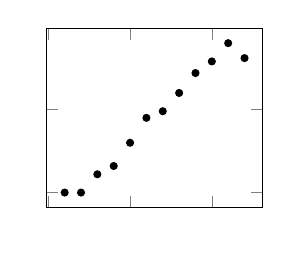
\begin{tikzpicture}
        \begin{axis}[%
            scale=0.4,
            yticklabels={,,},
            xticklabels={,,},
            scatter/classes={a={mark=*,draw=black,mark size=1.25pt,}}
        ]
            \addplot[scatter,only marks,scatter src=explicit symbolic]%
                table[meta=label,row sep=\\] 
            {
                x y label\\
                1 5 a\\
                2 5 a\\
                3 6.1 a\\
                4 6.6 a\\
                5 8 a\\
                6 9.5 a\\
                7 9.9 a\\
                8 11 a\\
                9 12.2 a\\
                10 12.9 a\\
                11 14 a\\
                12 13.1 a\\
            };
        \end{axis}
    \end{tikzpicture}
}
{
    \centering
    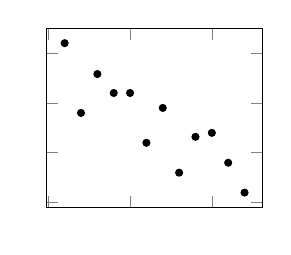
\begin{tikzpicture}
        \begin{axis}[%
            scale=0.4,
            yticklabels={,,},
            xticklabels={,,},
            scatter/classes={a={mark=*,draw=black,mark size=1.25pt,}}
        ]
            \addplot[scatter,only marks,scatter src=explicit symbolic]%
                table[meta=label,row sep=\\] 
            {
                x y label\\
                12 1 a\\
                11 4 a\\
                10 7 a\\
                9 6.6 a\\
                8 3 a\\
                7 9.5 a\\
                6 6 a\\
                5 11 a\\
                4 11 a\\
                3 12.9 a\\
                2 9 a\\
                1 16 a\\
            };
        \end{axis}
    \end{tikzpicture}    
}